
\chapter{Machine Learning}\label{Machine Learning}

Machine learning is een welbekend begrip in de informatica wereld, maar wat het juist omvat, welke algemene technieken er bestaan en met welke factoren men dient rekening te houden, wordt besproken in dit hoofdstuk.

\section{Wat is Machine Learning}\label{Wat is Machine Learning}

Over Machine Learning bestaat nergens een eenduidige definitie. Velen hebben geprobeerd om een eenduidige definitie te defini\"eren. \citet{samuel2000some} definieerde machine learning als:
\newline
\newline
\textit{Field of study that gives computers the ability to learn without being explicitly programmed}.
\newline
\newline
Later stelde \citet{mitchell1997machine} een well-posed learning problem als 
\newline
\newline
\textit{A computer program is said to learn from experience E with respect to some class of tasks T and performance measure P, if its performance at tasks in T, as measured by P, improves with experience E.}
\newline
\newline
%
We nemen een damspel als voorbeeld. De ervaring $E$ omschrijven we het best als de data die het computer programma als input krijgt. Met als toepassing het damspel stellen we de ervaring gelijk aan duizend spelletjes waarin alle data in zit zoals bijvoorbeeld welke stappen de speler en tegenspeler hebben gezet tijdens het spel. De taak $T$ van het computerprogramma is dammen. Het leren van het dammen wordt afgewogen tegenover de prestatie. Het doel van een damspel is het spel winnen dus de prestatie $P$ is het winnen of verliezen van het spel. De computer kan uit de data en aan de hand van de prestatie van ieder spel afleiden, wat goede zetten zijn en welke niet. Deze afleiding kan gebeuren aan de hand van kansvoorspelling en de score functie. De score functie is een functie die de nauwkeurigheid meet van een voorspelling. Het gaat aan iedere voorspelling een score toewijzen, hoe hoger de score, hoe hoger de nauwkeurigheid. We trachten altijd  de voorspelling te nemen met de grootste score. Wat betekent dat die voorspelling het meest correct is. Door telkens bij iedere zet alle mogelijke zetten en hun overwinningskrans bij te stellen door de score functie en telkens de zet te selecteren met de grootste overwinningskansen, kan het programma zich telkens verbeteren in het dammen. Als we ons voorbeeld nu defini\"eren in de woorden van Tom Mitchell, kunnen we zeggen dat het computerprogramma leert dammen uit duizend spelletjes en zich per spel telkens gaat verbeteren op basis van winst en verlies.\\    
Algemeen omschrijft men machine learning het best als een onderzoeksdomein dat zich bezighoudt met het onderzoeken en de ontwikkeling van zelflerende algoritmes. Hoofdzakelijk bestaat machine learning uit drie stappen namelijk data verzamelen, verwerken en analyseren.
\newline
Binnen machine learning onderscheidt men verschillende groepen van lerende algoritmen. Zo heeft men supervised learning, unsupervised learning, reinforcement learning en recommender systems. In deze voorbereiding legt men zich enkel op supervised en unsupervised learning. Deze soorten algoritmen omvatten specifiekere technieken die zich lenen tot het gebruik bij text mining.


\section{Supervised Learning}\label{Supervised Learning}

In machine learning beschikken we vaak over een dataset, ook wel trainingsset genoemd, met voorbeelden over het concept dat we willen aanleren. Bij supervised learning bevat de trainingsset input-output waarden ($x_{1},x_{2},...,x_{d},y$). De $x_{i}$ stelt alle inputwaarden of features voor en $y$ de outputwaarde. Bij supervised training is de mapping van bepaalde inputwaarden op een bepaalde output waarde aanwezig in de dataset. In de Machine Learning hebben algoritmes als doel een hypothese of model te vormen over deze mapping. Dit is ook het geval bij supervised learning.Met de hypothese, bijvoorbeeld de functie $y=f(x_{1},x_{2},...,x_{d}$, kan men nieuwe input-output waarden voorspellen. Als de inputwaarden $x_{i}$ gekend zijn kan men de outputwaarde $y$ van het nieuwe paar voorspellen aan de hand van de hypothese.  
\newline
Als voorbeeld een trainingsset met positieve en negatieve artikels nemen. Van ieder artikel in de dataset weten we of het positief of negatief is. De mapping van een het artikel ofwel een hoop woorden naar het concept \textit{positief} of \textit{negatief} wordt gebruikt door het algoritme om een hypothese te bepalen. De vele woorden zijn de inputwaarden $x_{i}$ en positief en negatief zijn de mogelijkheden voor de outputwaarde $y$. Uiteindelijk zal het algoritme zelfstandig kunnen beslissen of een gegeven willekeurig artikel positief of negatief is aan de hand van zijn hypothese.
\newline
In ons voorbeeld hebben we enkel positief en negatief als keuze voor onze outputwaarde $y$. Een ander voorbeeld is een spamfilter waarbij we classificeren tussen spam en geen spam. Wanneer we een hypothese opstellen voor een kleine set aan mogelijkheden voor de outputwaarde $y$, zoals onze spamfilter of onze artikels, spreekt men van een \textbf{\textit{classificatie probleem}}. Wanneer $y$ tot een hele grote of zelfs oneindige groep behoord en we daar een hypothese voor opstellen, spreekt men van een \textbf{\textit{regressie probleem}} bijvoorbeeld het bepalen van de huisprijs aan de hand van de bewoonbare oppervlakte.

\subsection{Regressie Probleem}\label{Regressie Probleem}

Zoals eerder vermeld is het doel van supervised learning om een hypothese op te stellen zodanig dat men voor inputwaarden $x_{i}$ outputwaarde $y$ kan bepalen. Een regressie probleem doet zich voor wanneer de outputwaarde $y$ continue, oneindig of een heel groot bereik aan mogelijkheden kan zijn. We illustreren het probleem met een voorbeeld, neem de prijsvoorspelling van een huis. 
In dit voorbeeld is onze ervaring $E$ de dataset $v$. De dataset $v$ bevat een mapping van de oppervlakte $x_{i}$ van het huis naar de prijs van het huis $y_{i}$. De taak T van het algoritme is de prijzen van huizen voorspellen op basis van hun oppervlakte. De prestatie $P$ wordt bepaald door een gegeven gemiddelde afwijking $\Theta$ van de echte prijs. Het algoritme stelt een hypothese op met de gegeven gemiddelde afwijking. Men kan de hypothese als volgt voorstellen:
\[ f(x_{i},\theta) = y_{i} \] 
\newline
We plotten nu de input-output waarden $(x_{i},y{i})$ op een grafiek.
\newline
%%TEKENENING HIER EEN GRAFIEK MET DATAPUNTEN 
\begin{center}
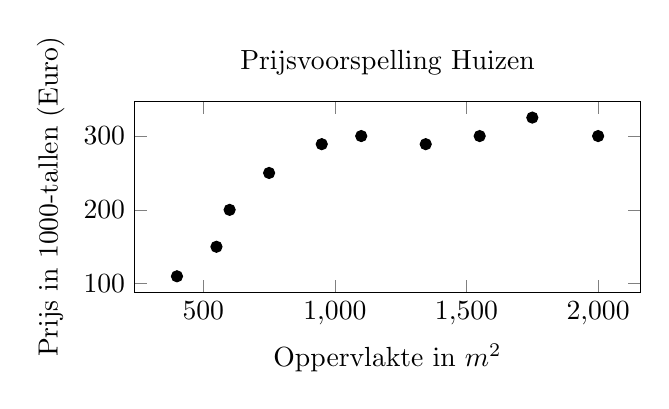
\begin{tikzpicture}
\begin{axis}[%
xlabel={Oppervlakte in $m^2$},
ylabel={Prijs in 1000-tallen (Euro)},
title={Prijsvoorspelling Huizen},
scatter/classes={%
    a={mark=o,draw=black}},
     width=8cm,
        height=4cm]
\addplot[only marks] table[row sep=\\] {
x y\\
400 110\\
550 150\\
600 200\\
750 250\\
950 289\\
1345 289\\
1550 300\\
1750 325\\
2000 300\\
1100 300\\};
\end{axis}
\end{tikzpicture}
\end{center}
\newline
%
 We kunnen aan de hand van de grafische weergave al een idee krijgen hoe onze hypothese of model er gaat uit zien. We kunnen zowel een lineair model als een polynomisch model opstellen. Bij een lineair model spreekt men van een verband tussen een scalaire afhankelijke variable $Y$ en onafhankelijke variable(n) $x$. Wanneer men dit plot krijgt men een rechte. Een lineair model heeft volgend functievoorschrift.
%
\[Y =  \theta_{n}x_{n} + \theta_{n}x_{n-1} + ... + \theta_{1}x_{1} + \theta_{0}\]
%
In ons voorbeeld hebben we maar \'e\'en inputwaarde namelijk de oppervlakte, dus ons voorschrift van onze hypothese heeft maar \'e\'en onafhankelijk variable x.
\newline
\[ Y = \theta_{1}x_{1} + \theta_{0}\] \\ 
\begin{center}
\begin{tikzpicture}
\begin{axis}[%
xlabel={Oppervlakte in $m^2$},
ylabel={Prijs in 1000-tallen (Euro)},
title={Prijsvoorspelling Huizen},
scatter/classes={%
    a={mark=o,draw=black}},
     width=8cm,
        height=4cm]
\addplot[only marks] table[row sep=\\] {
X Y\\
400 110\\
550 150\\
600 200\\
750 250\\
950 289\\
1345 289\\
1550 300\\
1750 325\\
2000 300\\
1100 300\\
};
\addplot table[row sep=\\,
    y={create col/linear regression={y=Y}}] 
    {
X Y\\
400 110\\
550 150\\
600 200\\
750 250\\
950 289\\
1345 289\\
1550 300\\
1750 325\\
2000 300\\
1100 300\\
};

\end{axis}
\end{tikzpicture}
\end{center}
\newline
%
%
De $\theta's$ zijn zo bepaald dat de hypothese of het model voldoet aan de vooropgelegde gemiddelde afwijking van de echte prijs. Andere waarden van $\theta's$ zorgen voor een andere  hypothese, maar alle hypotheses blijven lineair. De techniek waarbij we een hypothese proberen op te stellen gebaseerd op een lineaire verband, noemt men \textbf{\textit{lineaire regressie}}. 
%
Als we terugkijken naar onze grafiek met gekende datawaarden, zien we ook dat we onze hypothese als een 2de graads veelterm kunnen zien. Als we dit plotten krijgen we een parabool. Bij een 2de graads of in het algemeen n-de graads veelterm model bestaat er een relatie tussen de afhankelijke variable $Y$ en de onafhankelijke variable(n) $x$ waarbij deze gemodelleerd worden als een n-de graad veelterm.
%
\[Y = \theta_{n}x^{n}_{n} + \theta_{n-1}x^{n-1}_{n-1} + .... +  \theta_{1}x_{1} + \theta_{0} \]
%
Zoals bij het lineaire model, we hebben maar \'e\'en inputwaarde dus we stellen een 2de graads veelterm
%
Onderstaande afbeelding toont hoe onze hypothese eruit kan zien als een 2de graads veelterm.
\begin{center}
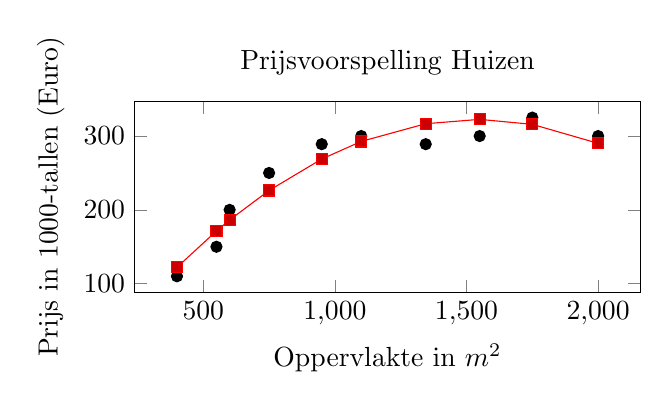
\begin{tikzpicture}
\begin{axis}[%
xlabel={Oppervlakte in $m^2$},
ylabel={Prijs in 1000-tallen (Euro)},
title={Prijsvoorspelling Huizen},
scatter/classes={%
    a={mark=o,draw=black}},
     width=8cm,
        height=4cm]
\addplot[only marks] table[row sep=\\] {
X Y\\
400 110\\
550 150\\
600 200\\
750 250\\
950 289\\
1345 289\\
1550 300\\
1750 325\\
2000 300\\
1100 300\\
};
\addplot table[row sep=\\] 
    {
X Y\\
400  122.1471267\\
550  171.4080927\\
600  186.2874525 \\
750  226.3026453\\
950  268.8695001\\
1100 292.7045896\\
1345 316.7225741\\
1550 322.6038785\\
1750 315.8599426\\
2000 290.0941979\\
};
\end{axis}
\end{tikzpicture}
\end{center}
\newline
%
Eveneens zijn de $\theta's$ hier zo bepaald dat de hypothese of het model voldoet aan de vooropgelegde gemiddelde afwijking van de echte prijs. Andere waarden van $\theta's$ zorgen voor een andere  hypothese, maar alle hypotheses blijven polynomisch. De techniek waarbij we een hypothese proberen op te stellen gebaseerd op een polynomisch verband, noemt men \textbf{\textit{polynoom regressie}}. 
\newline
In deze voorbereiding gaan we ons enkel verder toespitsen op lineaire regressie. 
%eventueel nog zeggen waarom

\subsubsection{Lineaire regressie}\label{lineaire regressie}

We hebben tot zo ver gezien dat een hypothese opstellen waarbij voor output $Y$ een hele reeks aan mogelijkheden voor een regressie probleem zorgt. Verder zeggen we dat men dit probleem kan oplossen door lineaire regressie. Dit houdt in dat men een hypothese opstelt op basis van een lineair verband.
%
Ter illustratie van een mogelijk lineair verband kijken we terug naar ons voorbeeld over de prijsvoorspelling van een huis op basis van de oppervlakte waarbij de hypothese wordt bepaald door lineaire regressie als:
\[H_{\theta}(x) = \theta_{1}x + \theta_{0}\]
%
Het laatste wat nog bepaald moet worden zijn de $\theta's$. Door verschillende waarden te nemen voor de $\theta's$, kan men verschillende hypotheses opstellen. Merk op dat de verschillende hypotheses steeds lineair blijven. Het bepalen van de waarden voor de $\theta's$, introduceert het minimalisatie probleem. Men wil de $\theta's$ zodanig bepalen dat de hypothese de kleinste gemiddelde afwijking van de resultaten geeft. Om dit minimalisatie probleem op te lossen gaat men gebruik maken van een kost functie  waarbij men het minimum van deze functie berekent door gradi\"ent afdaling. De kost functie is een functie die voor bepaalde theta's de gemiddelde afwijking van de echte waarden, ook wel kost genoemd, gaat berekenen.  



\subsubsection{Kost Functie en Gradi\"ent afdaling}\label{Kost Functie en Gradule afdaling}

We willen een zo goed mogelijke hypothese opstellen. Men heeft een goede hypothese wanneer de gemiddelde afwijking van de outputwaarden ten opzichte van de echte waarden, zo laag mogelijk is. Die gemiddelde afwijking van een hypothese noemen we ook de kost. Verder zien we dat we voor andere waarden van de $\theta's$ een andere hypothese krijgen en dus ook telkens een andere kost. Door een kost functie op te stellen waarbij de parameters de $\theta's$ zijn en de output de kost, kan men bepalen voor welke $\theta's$ de kost het laagste is. Deze $\theta$-waarden gebruikt men dan voor het uiteindelijke functievoorschrift van de hypothese. \\
Als we ons voorbeeld van de prijsvoorspelling van huizen er terug bij nemen, waarbij we de hypothese gaan opstellen aan de hand van lineaire regressie stellen we de kost functie als volgt op\\
%%FORMULE DE KOST FUNCTIE
\[J(\theta_{0},\theta_{1}) = \frac{1}{2m}\sum_{i=1}^{m} (H_{\theta}(x_i) - Y_i )^2\]
met als model 
\[H_{\theta}(x) = \theta_{1}x + \theta_{0}\]
%
Deze kost functie noemt men ook wel de \textbf{\textit{squared error cost function}}. Merk op dat we niet zomaar telkens de som van het verschil tussen het resultaat van de hypothese nemen en de eigenlijke waarden. Het kwadraat van het verschil wordt genomen vanwege de negatieve verschillen die ook moeten worden opgenomen als afwijking. Verder vereenvoudigt men het rekenwerk door te delen door twee (deling door 2 zorgt ervoor dat factor 2 wegvalt in de gradient). 
\newline
Zoals eerder gezegd is het de bedoeling om de waarden van de $\theta's$ te bepalen zodanig dat onze kost zo klein mogelijk is. Om het minimum van de kost functie te vinden, gebruiken we de techniek \textbf{\textit{gradi\"ent afdaling}}. Omwille van verschillende redenen is gradi\"ent afdaling een populaire techniek binnen machine learning voor minimalisatie. Algemeen werkt de techniek voor een algemene kost functie met n parameters J($\theta_{0},\theta_{1},\theta_{2},\theta_{3}, ... ,\theta_{n}$). Gradi\"ent afdeling heeft altijd een oplossing aangezien lineaire regressie met kwadratische kost altijd \'e\'en globaal minimum heeft en gradi\"ent afdaling altijd een minimum kan vinden.
Op onderstaande afbeelding ziet men een grafische weergave van de kost functie $J(\theta_{0},\theta_{1})$ van de huisprijsvoorspelling.
\newline
%AFBEELDING VAN EEN 3D-PLOT
%beschrijving: van axissen
\begin{center}
  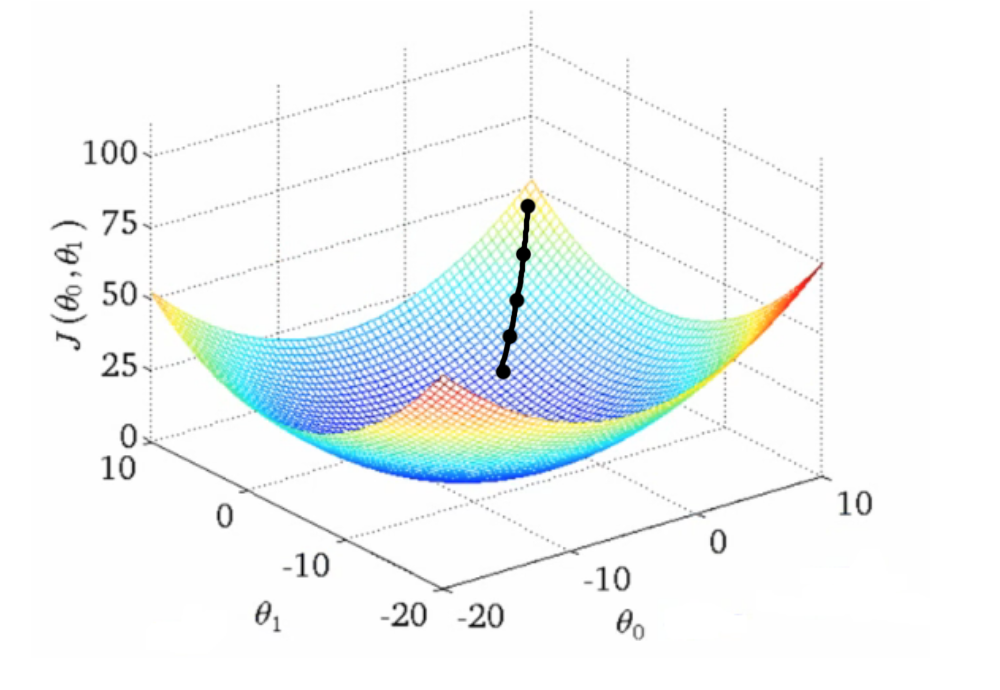
\includegraphics[width=5cm]{3d_plot_1}
  \captionof{figure}{Weergave van de kost functie (Bron:\url{https://class.coursera.org/ml-005/lecture/preview)}}
\end{center}
%
 Het principe van gradi\"ent afdaling is vrij intu\"itief en staat ook aangeduid op bovenstaande tekening door de zwarte lijn. Het start met een random start punt, vervolgens gaat men stapsgewijs proberen te dalen tot het convergeert naar een lokaal minimum. Men kijkt bij iedere stap of de huidige kost kleiner is als de vorige. Zo ja, dan wil dit zeggen dat de kost nog altijd daalt en nog geen minimum gevonden is. Indien de huidige kost groter is, dan weet het algoritme dat het niet meer daalt en er een minimum gevonden is.
\newline
De werking van gradi\"ent afdaling kunnen we formeel neerschrijven. Met onze eerder opgestelde hypothese $H_{\theta}(x)$ en kostfunctie $J(\theta_{0},\theta_{1})$ noteren we het stapsgewijs dalen als \\
%%FORMULE STAPGEWIJS DALEN
\[ \theta_{j} := \theta_{j} - \alpha\frac{d}{d\theta_{j}}J(\theta_{0},\theta_{1})   \text{  (voor j = 0 en j = 1)}\] 
\newline
$\alpha$ noemt men de learning rate. Dit is de grootte van de stappen die men neemt bij het afdalen. De learning rate is een belangrijk element in het gradi\"ent afdalingsalgoritme. Als men deze te groot neemt kan men lokale minima overslagen en convergeert het algoritme niet. Als men $\alpha$  te klein neemt, zal het algoritme heel lang duren. 
\newline
Een belangrijk detail bij de formule en het algoritme is het simultaan updaten van de twee parameters (zowel $\theta_{0}$ als $\theta_{1}$). Als men dit niet doet, spreekt men niet van gradi\"ent afdaling.
\newline
Soms kan het zijn dat men gradi\"ent afdaling moet toepassen op een kostfunctie met meerdere lokale minima bijvoorbeeld bij neurale netwerken. Dit kan voor problemen zorgen. Het algoritme zal stoppen in deze lokale minima en men wil het absolute minimum als eindresultaat. Meerdere keren het algoritme uitvoeren met een andere startpunt, verkleint de kans dat het uiteindelijke resultaat van de gradi\"ent afdaling een lokaal minimum is. Onderstaande afbeelding illustreert dit.
\begin{center}
  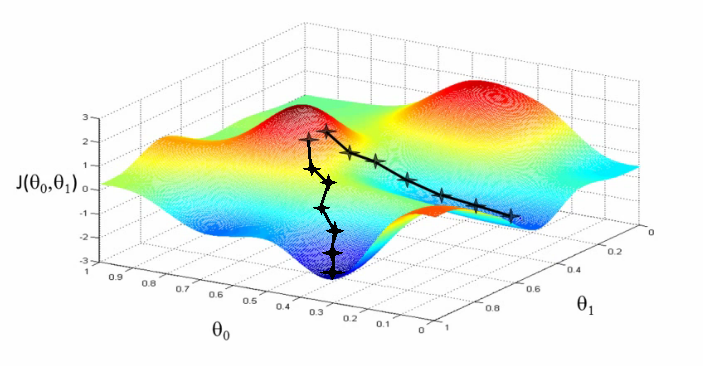
\includegraphics[width=5cm]{3d_plot}
  \captionof{figure}{kost functie met meerdere lokale minima. (Bron:\url{https://class.coursera.org/ml-005/lecture/preview})}
\end{center}
Nu dat we het regressie probleem bij supervised learning hebben afgehandeld, gaan over naar het classificatie probleem. Zoals eerder vermeld is het classificatie probleem verschillend van het regressie probleem door dat men inputwaarden moet mappen op een outputwaarde die behoort tot een kleine set van mogelijkheden. Bij het regressie probleem kan de outputwaarde behoren tot een oneindige of grote reeks van mogelijkheden.

\subsection{Classificatie Probleem}\label{Classificatie Probleem}

Een classificatie probleem is een ander probleem dat zich voordoet bij supervised learning. Men spreekt van een classificatie probleem wanneer men een hypothese moet opstellen waarbij de output van de hypothese behoort tot een kleine discrete set van mogelijkheden. Neem als voorbeeld een spamfilter, waarbij spam en geen spam de enigste mogelijke outputwaarde zijn. De experience $E$ is een dataset $v$ met mails. We hebben te maken met supervised learning, dus de dataset bevat voorbeelden met welke mails spam zijn en welke niet. De taak $T$ van de spamfilter is bepalen welke mails behoren tot spammail en welke niet. De prestatie $P$ wordt beoordeeld op basis van de kost bijvoorbeeld hoeveel mails er fout zijn gesorteerd.
\newline
Een re\"eel gevaar bij classificatie aan de hand van voorbeelden is overfitting en underfitting.
\citet{mitchell1997machine} definieert overfitting als volgt:
\newline
\newline
\textit{Given a hypothesis space H , a hypothesis h E H is said to overfit the training data if there exists some alternative hypothesis h' E H, such that h has smaller error than h' over the training examples, but h' has a smaller error than h over the entire distribution of instances.}
\newline
\newline
Wat eigenlijk wil zeggen dat hypothese H te goed werkt op zijn eigen trainingsset, maar vanaf het andere waarden begint te classificeren is de prestatie veel minder. Bij underfitting is het juist omgekeerd. De prestatie is lager op de trainingsset dan op een grote nieuwe dataset.
%
Een populaire methode om een classificatie probleem op te lossen is \textbf{\textit{logistische regressie}}

\subsubsection{Logistische Regressie}\label{Logistische Regressie}

Het classificatie probleem is verschillend van het regressie probleem door dat de output behoort tot een kleine discrete set van outputmogelijkheden. Logistische regressie gaat in principe outputwaarden omvormen zodanig dat met het classificatie probleem kan oplossen met lineaire regressie. We zagen dat de hypothese volgens een lineaire regressie er als volgend uit zag:
\[ H_{\theta}(x_{n}, x_{n-1},...,x_{1}) = \theta_{n}x_{n} + \theta_{n-1}x_{n-1} + ... + \theta_{1}x_{1} + \theta_{0}  \] 
%
Verkort kunnen we dit schrijven als een matrixvermenigvuldiging van de co\"effici\"enten $(\theta_{n},\theta_{n-1},...,\theta_{1})$ en de inputwaarden $(x_{n},x_{n-1},...,x_{1})$

\[ H_{\theta}(x) = (\theta^{T}x)\] 
%
De hypothese bij logistische regressie ziet er hetzelfde uit, enkel wordt de \textbf{sigmo\"ide functie} of logistische functie toegepast.
\[ H_{\theta}(x) = g((\theta^{T}x))\]
%
met als sigmo\"ide functie
%
\[g(z) = \frac{1}{1 + e^{-z}}  \text{  (z is een ree\"el getal)} \]
\newline
\newline
\begin{figure}[h]
\centering
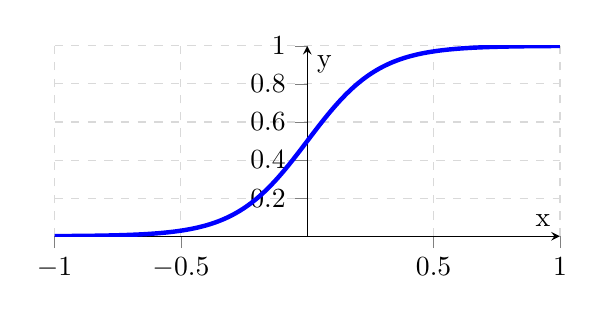
\begin{tikzpicture}
    \begin{axis}[
        legend pos=north west,
        axis x line=middle,
        axis y line=middle,
        grid = major,
        width=8cm,
        height=4cm,
        grid style={dashed, gray!30},
        xmin=-1,     % start the diagram at this x-coordinate
        xmax= 1,    % end   the diagram at this x-coordinate
        ymin= 0,     % start the diagram at this y-coordinate
        ymax= 1,   % end   the diagram at this y-coordinate
        %axis background/.style={fill=white},
        xlabel=x,
        ylabel=y,
        tick align=outside,
        enlargelimits=false]
      % plot the stirling-formulae
      \addplot[domain=-1:1, blue, ultra thick,samples=500] {1/(1+exp(-7*x))};
    \end{axis} 
\end{tikzpicture}
\captionof{figure}{illustratie van een sigmo\"ide functie.}
\end{figure}
\newline

De sigmo\"ide functie is een S-vormige functie en zorgt er voor dat iedere inputwaarden $(x_{1}, x_{2} , ... , x_{n})$ gemapt worden op \'e\'en van de outputwaarde $y$ uit de discrete set van mogelijkheden. Neem even terug het voorbeeld van de spamfilter. Elke mail moet ofwel spam zijn ofwel geen spam. De hypothese voor logistische regressie kan men uiteindelijk uitgeschrijven als
%
\[ g(z) = \frac{1}{1 + e^{-\theta^{T}x}} \]
%
Als we de functie $Z (= \theta^{T}x)$ plotten samen met de resultaten van de hypothese, komt $Z$ overeen met een beslissingslijn. Een beslissingslijn geeft de grens weer tussen twee verschillende klassen. 
Bijvoorbeeld in onderstaand voorbeeld is een dataset van mails weergegeven met de beslissingslijn $Z$. Alles onder de beslissingslijn is geen spam, alles erboven wel. \\
%
\begin{center}
  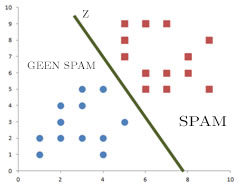
\includegraphics[width=5cm]{decissionline}
  \captionof{figure}{illustratie van een mogelijke beslissingslijn.}
\end{center}
%
Doordat de hypothese buiten de sigmo\"ide functie overeenkomt met lineaire regressie, gelden dezelfde principes. We zoeken naar een model waarbij de kost zo laag mogelijk is. Andere waarden voor van $\theta's$ geven andere hypotheses maar het lineair verband blijft. De uiteindelijke hypothese dat we moeten hebben, is diegene waarbij de kost het laagst is. Bij ons voorbeeld over spamfilters is dit de hoeveelheid mails die fout gesorteerd zijn. Dit minimalisatie probleem kunnen we wederom oplossen door de kost functie en gradi\"ent afdaling.

\section{Unsupervised Learning}\label{Unsupervised Learning}

Unsupervised learning is een techniek waarbij het algoritme zelfstandig moet leren hoe de mapping verloopt tussen de inputwaarden en de outputwaarde. Bij supervised learning bevat de trainingsset voorbeelden van input-output waarden $(x_{1},x_{2},...,x_{d},y)$, en gebruikt het algoritme deze voorbeelden om een hypothese op te stellen zodat het nieuwe input-output waarden kan voorspellen. Dit is niet het geval bij unsupervised learning, de gegeven dataset bevat deze voorbeelden niet en het algoritme moet op een andere manier een hypothese opstellen. De trainingsset bevat niet de antwoorden.
\newline
Men probeert structuren en patronen te herkennen in de dataset en aan de hand hiervan een hypothese op te stellen. Het herkennen van structuren en patronen en dan juist identificeren doet men aan de hand van cluster algoritmes. Concreet gaat een cluster algoritme de data groeperen of \textbf{\textit{clusteren}} in groepen en zo de data concreet identificeren. Onderstaand voorbeeld illustreert hoe deze identificatie kan verlopen.\\
\begin{center}
  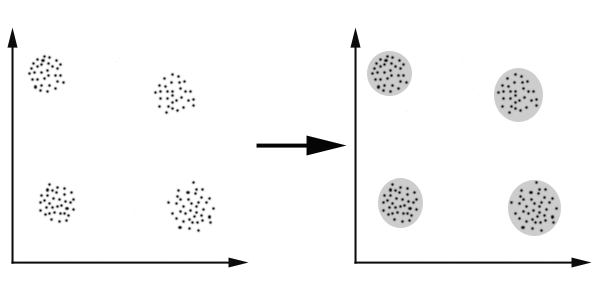
\includegraphics[width=5cm]{clustering}
  \captionof{figure}{Identificatie bij clustering (Bron:\url{http://home.deib.polimi.it/matteucc/Clustering/tutorial_html/index.html}}
\end{center}
\newline
We gaan niet verder in op unsupervised learning. Het is minder toepasselijk in verband met text mining.
